\documentclass{proc}
\usepackage{url}
\def\UrlBreaks{\do\/\do-}
\usepackage{graphicx, subcaption}
\usepackage{epstopdf}
\usepackage{eso-pic}
\usepackage{picture}
\usepackage{listings}
\usepackage{tabu}
\linespread{1.2}
\definecolor{grey}{rgb}{0.96, 0.96, 0.96}
\lstset {
  backgroundcolor=\color{grey},
  linewidth=160mm,
  basicstyle=\footnotesize\ttfamily, % Global Code Style
  columns=fixed, % make all characters equal width
  showstringspaces=false, % lets spaces in strings appear as real spaces
  breaklines=true, % wrap lines if they don't fit
  rulecolor=\color{grey},
  moredelim=**[is][\color{blue}]{@}{@},
}



\begin{document}

\title{GlassBox: Fault-Tolerant Host Monitoring on Commodity Operating Systems}

\author{Brett Jia \hspace{1em} Jennifer Bi}

\maketitle

\section*{Abstract}

In modern computer systems, administrators, developers, and users often desire to monitor their operating systems for usage metrics, such as filesystem usage, CPU utilization, RAM utilization, and others. In other cases, systems administrators and developers may be interested in monitoring log files on production machines to gauge the health and execution of live applications. Monitoring can be done through automated software that report metrics to a metrics aggregator, or through a user manually running certain tools that probe the operating system for data. In either case, the system could be at risk of damage and compromise from buggy or malicious software and user negligence or error. To address this problem, we present an approach to running host monitoring tools in containers with a read-only view of the surrounding system, guaranteeing fault tolerance and protection to the host system's stability.

\section*{1. Introduction}

Despite the best efforts of software designers and system administrators, a major weakness of system administration and system monitoring is the reliance on bug-free software and perfect user execution. While some system monitoring tools such as \texttt{ps} do not require elevated privileges and rely on reading deprivileged virtual filesystem objects exposed by the operating system kernel via the \texttt{proc} mount, other tools such as \texttt{lsof} require superuser privileges to display full metrics on a system's open file descriptors by reading protected files in the same \texttt{proc} mount. Especially for the case of tools requiring superuser privileges, any system administration or system monitoring task could potentially be destructive to the host system through malicious software or user error if incorrect commands and arguments are executed, resulting in the expenditure of hours and money to restore the system and its contents to a state prior to disaster.

Aside from monitoring of host system data and statistics, often system administrators and developers alike desire to monitor interesting files on a machine's filesystem for tracing the execution of a running application or troubleshooting software. Files such as \texttt{/var/log/messages} and application runtime logs provide a wealth of information about the health and execution of the system and live applications running on the host, and these logs can be used in a chain of standard Unix commands (such as \texttt{grep} and \texttt{sort}) to provide useful metrics and analysis. Similar to the risks of running system monitoring tasks, even accessing log files directly on the machine (whether using a privileged user or not) can jeopardize the health and stability of the host and the applications running on the host by accidentally crashing applications or starving the host of resources by spending too much computing resources on log file analysis.

An early solution to the problem of fault tolerance is to utilize virtual machines to guarantee isolation between processes \cite{garfinkel2003terra}. However, while virtual machines can indeed be used to provide an isolated environment for untrusted code execution \cite{wen2012virtualization}, recent performance comparisons between hypervisor-based virtualization and container-based (i.e. lightweight or kernel-based) virtualization show that virtual machines exhibit more overhead with certain workloads when compared to kernel-supported container mechanisms \cite{felter2014docker, morabito2015hypervisors}.

Instead of fault tolerance through hardware virtualization by way of virtual machines, recent work has emphasized ensuring fault tolerance through operating system virtualization \cite{soltesz2007container}. An early approach to operating system virtualization introduces a kernel interposition method to restrict an application's access to certain system calls (syscalls), as implemented in Janus \cite{goldberg1996janus} and later in MBOX \cite{kim2013mbox}. Other sandboxing mechanisms have been introduced, including new system calls to create kernel-supported process isolation called jails \cite{kamp2000jails}, new filesystem tools leveraging \texttt{mount} and \texttt{chroot} to restrict filesystem access \cite{prevelakis2001fmac}, namespace isolation to create kernel-supported process containers \cite{biederman2006namespaces, menage2007containers}, and control groups (\textit{cgroups}) to limit resource consumption of a group of processes \cite{menagecgroups}.

Modern containers combine these operating system virtualization approaches to create lightweight isolated execution contexts. The industry standard choice for Linux container technology is Docker, which combines Linux \textit{cgroups}, \textit{namespaces}, \textit{capabilities}, and more using its custom container runtime, \textit{libcontainer} \cite{hykes2014libcontainer}. With the formation of the Open Container Initiative (OCI) in 2015 \cite{opencontainerinitiative}, the design and construction of container platforms became standardized with OCI's \textit{runtime-spec} and \textit{image-spec}, providing a framework for distributors to develop their own cross-compatible container implementations.

In our research, we present \textit{GlassBox}, a container-based system to provide fault-tolerance and fault-containment semantics to host monitoring processes on commodity Linux operating systems. \textit{GlassBox} addresses the problems of host stability and fault tolerance that arise from executing buggy or compromised system tools and from user negligence and error when performing system administration tasks and application log monitoring through the use of modern container technologies. In the following sections, we first present background on containers and existing container technologies, then discuss a theoretical view of the host resources a fault-tolerant host monitoring system should allow access to and the resources the system should protect, then discuss representative Linux tools and the host resources they require for accurate system monitoring, then discuss the prototype architecture and implementation of \textit{GlassBox}, and close with a discussion of functionality and future work.

\section*{2. Containers}

Linux supports the creation of isolated filesystem environments through \texttt{chroot} jails and \texttt{mount} namespaces. While \texttt{chroot} changes the root filesystem directory for a process, \texttt{mount} namespaces allow for flexibility of what directory the process sees as the filesystem root and security of the overall filesystem on the host. Bind mounts (\texttt{mount} command with the \texttt{--bind} option) in particular make a subset of a host's filesystem visible at a second mount point \cite{bindmount}, with the option of mounting it as ``read-only.'' This kind of ``symbolic link'' allows for a specific view of the filesystem namespace. By bind mounting the root directory or \texttt{/proc}, host information becomes readable by a jailed process otherwise closed off from the filesystem. Indeed, bind mounts can currently be used with Docker containers to provide visibility to certain files on the host filesystem while keeping the containers' stong isolation guarantees \cite{dockerdoc}.

Host-monitoring applications isolated in read-only filesystems may also need a place to temporarily store the output of its monitoring. \texttt{tmpfs} can be used to store temporary data in RAM rather than on disk. Furthermore, the size can be limited to prevent a host-monitoring program from consuming too much memory. When combined with Docker, a \texttt{tmpfs} mount is persisted in host memory while the container runs, and removed when a container stops.

Linux also supports syscall filtering via \texttt{seccomp-bpf} filters, which are used in conjunction with other container primitives to implement containerization in Docker, LXC, etc. Currently, the container runtime \textit{runC} (built on its predecessor \textit{libcontainer} \cite{hykes2014libcontainer}) uses \texttt{seccomp-bpf} to perform syscalls interposition \cite{opencontainerinitiative}. The rule-based filtering of existing \texttt{seccomp-bpf} in Linux, however, does not allow for more advanced access control policy validation or syscall emulation \cite{seccompuserspace}.

Commercial container solutions such as Docker and rkt offer pre-built networking options to faciliate networking connectivity between the container and the host \cite{dockernetworking, rktnetworking}. The two general categories of network connectivity offered are \textit{host} and \textit{container}, both built on the network separation properties provided by Linux network namespaces. \textit{Host} network configurations set up the container to share the same network namespace as that of the calling process, effectively giving the container the same network access and network configuration as the parent process. \textit{Container} network configurations create a separate network namespace for the container, separating its connectivity from the network namespace of the parent process. In \textit{container} network configurations, a network bridge and virtual ethernet devices are used to connect the container's network with the host, effectively exposing the container as a new ``host'' connected to the host machine.

CPU and memory usage can also be restricted in existing container solutions through the use of Linux capabilities and \textit{cgroups} \cite{dockerconstraints}. As \textit{cgroups} function to group a set of processes under the same ``control group'' for broad resource control and process management \cite{menagecgroups}, container implementations such as Docker use \textit{cgroups} to fine-tune the memory and CPU-time allowances of the group of processes running in a container. Additionally, Linux capabilities can be used to give the container permission to modify its process scheduler directly in the host kernel, such as setting \textit{nice} values or use the Linux \textit{realtime} process scheduler.

\section*{3. Fault-Tolerant Host Monitoring}

We postulate that an ideal fault-tolerant host monitoring system should observe the following two characteristics:
\begin{enumerate}
    \item The system should be able to accurately view a subset of the host's state, both volatile (e.g. in-memory) and persistent (e.g. on-disk), as required by the information set the system is monitoring.
    \item The system's execution, both in normal and abnormal circumstances, must guarantee that stability of the host machine is maintained.
\end{enumerate}

An accurate view of the host's state is required for the host monitoring system to be useful. For example, the \texttt{top} program, which monitors system memory and CPU usage by process, requires access to volatile information to function correctly (in this case, the \texttt{/proc} virtual file system). It is easy to imagine that the \texttt{top} tool would not function correctly or be nearly as useful if \texttt{/proc} did not exist, or if reading from \texttt{/proc} yielded incorrect or invalid data.

On the other hand, a strong guarantee that the monitoring system's execution maintains the stability of the host machine is required to ensure fault-tolerance. We define the property of maintaining a host's \textit{stability} as ``preventing any modification of volatile and persistent data or usage of computing resources that could, now or in the future, alter the execution or responsiveness of the host or applications on the host.'' In other words, the monitoring system should ensure that it accesses memory and storage outside of the monitor in a strictly read-only fashion, should not send any signals or messages to existing processes, and should not starve the host of shared resources.

Traditionally, there is tension between these two requirements of accurate host monitoring and fault-tolerance. This tension can be easily exemplified by the tool \texttt{lsof}, which displays information about all of the host's open file descriptors by reading from the \texttt{/proc} filesystem. Running \texttt{lsof} with a non-superuser user can display some file descriptor information for processes running under the user, but is not permissioned to read information about processes running under other users. While executing \texttt{lsof} under a non-superuser user protects the host from harm if the \texttt{lsof} execution misbehaves or its binary has been compromised, it is clear that this protection is provided at the cost of losing access to certain information about the system. On the other hand, running \texttt{lsof} as a superuser would provide this information, but puts the host at significantly more risk if the \texttt{lsof} binary has been compromised.

\section*{4. Host-Monitoring Linux Tools}

 \begin{figure}[h]
\begin{tabular}{ |p{40mm}|p{30mm}| }
\hline
\textbf{Monitoring tool} &  \textbf{Resource}\\\hline
df (GNU coreutils)\newline 8.25-2ubuntu3{\raise.17ex\hbox{$\scriptstyle\sim$}}16.04  & disk\\\hline
du (GNU coreutils)\newline 8.25-2ubuntu3{\raise.17ex\hbox{$\scriptstyle\sim$}}16.04  &  disk\\\hline
ip (iproute2)\newline 4.3.0-1ubuntu3.16.04.4 &  network\\\hline
tcpdump\newline 4.9.2-0ubuntu0.16.04.1 &  network\\\hline
free (procps)\newline 2:3.3.10-4ubuntu2.4 &  memory\\\hline
ps (procps)\newline 2:3.3.10-4ubuntu2.4  & process\\\hline
pidstat (sysstat)\newline 11.2.0-1ubuntu0.2 & process\\\hline
sar (sysstat)\newline 11.2.0-1ubuntu0.2 &  system activity\\\hline
gkrellm\newline 2.3.6{\raise.17ex\hbox{$\scriptstyle\sim$}}rc1-1build1 & cpu, disk, process,\newline network interfaces\\\hline
wireshark (wireshark-qt)\newline 2.6.6-1{\raise.17ex\hbox{$\scriptstyle\sim$}}ubuntu16.04.0 & network\\\hline
vim\newline 2:7.4.1689-3ubuntu1.2 & text editor \\\hline
\end{tabular}
\caption{Selected Linux tools}
\end{figure}

 \begin{figure*}[t]
\begin{lstlisting}[linewidth=\linewidth]
% time     seconds  usecs/call     calls    errors syscall
------ ----------- ----------- --------- --------- ----------------
100.00    0.000120           0       243           read
  0.00    0.000000           0         1           write
  0.00    0.000000           0       257        12 open
  0.00    0.000000           0       245           close
  0.00    0.000000           0       125         4 stat
  0.00    0.000000           0        18           fstat
  0.00    0.000000           0         2           lseek
  0.00    0.000000           0        41           mmap
  0.00    0.000000           0        24           mprotect
  0.00    0.000000           0         1           munmap
  0.00    0.000000           0         3           brk
  0.00    0.000000           0        24           rt_sigaction
  0.00    0.000000           0         1           rt_sigprocmask
  0.00    0.000000           0         4         3 ioctl
  0.00    0.000000           0        13        13 access
  0.00    0.000000           0         1           execve
  0.00    0.000000           0         1           uname
  0.00    0.000000           0         2           getdents
  0.00    0.000000           0         4           readlink
  0.00    0.000000           0         1           getrlimit
  0.00    0.000000           0         1           geteuid
  0.00    0.000000           0         2         2 statfs
  0.00    0.000000           0         1           arch_prctl
  0.00    0.000000           0         1           futex
  0.00    0.000000           0         1           set_tid_address
  0.00    0.000000           0         1           set_robust_list
------ ----------- ----------- --------- --------- ----------------
100.00    0.000120                  1018        34 total
 \end{lstlisting}
 \caption{\texttt{strace -c ps} output}
\end{figure*}

 \begin{figure}[t]
\begin{lstlisting}[linewidth=\linewidth]
open("/proc/1926/stat", O_RDONLY)       = 6
open("/proc/1926/status", O_RDONLY)     = 6
open("/proc/1930/stat", O_RDONLY)       = 6
open("/proc/1930/status", O_RDONLY)     = 6
open("/proc/1932/stat", O_RDONLY)       = 6
open("/proc/1932/status", O_RDONLY)     = 6
open("/proc/1934/stat", O_RDONLY)       = 6
open("/proc/1934/status", O_RDONLY)     = 6
 \end{lstlisting}
 \caption{Truncated \texttt{strace ps} output}
\end{figure}

GlassBox provides monitoring tools running inside the container with access to certain host information required by the specific monitoring tasks performed. To provide correct functionality of the tools, we first need to know what information each one expects from the host system.

We used the Linux utility \texttt{strace} to retrieve a syscall profile for various common system monitoring tools, listed in Figure 1, to determine what host resources these tools require. These tools were selected to be representative of common host monitoring workloads seeking information about a host's filsystem and disk usage, network state and traffic, memory usage, process status, and general system activity. A common text editor, \texttt{vim}, was also selected as a representative tool for opening and reading application log files. In our investigation, \texttt{strace} version 4.11-1ubuntu3 was used running on a virtualized Ubuntu 16.04.6 LTS (Linux 4.4.0-145-generic) on VirtualBox 5.2.26 r128414. Graphical tools (such as \texttt{wireshark}) used the VcXsrv X server, version 1.20.1.4. Sample output of \texttt{strace} on the \texttt{ps} command can be found in Figure 2.

The output of \texttt{strace} informed us that the \texttt{ps} tool largely performs filesystem operations, since the majority of the system calls utilized are filesystem-related functions (such as \texttt{open}, \texttt{read}, and \texttt{stat}). Inspecting the actual system call arguments to the \texttt{open} function provided clarity to what files are being used. Figure 3 shows truncated output of \texttt{strace} with a filter on the \texttt{open} syscall name. We discovered similar findings from the programs \texttt{df}, \texttt{free}, \texttt{pidstat}, \texttt{sar}, and \texttt{gkrellm}, with the \texttt{df} tool also requiring access to the \texttt{statfs} system call.

Unlike the previous tools, the tool \texttt{du}'s \texttt{strace} profile used the system call \texttt{openat} instead of \texttt{open}, and appeared to use \texttt{openat} to recursively traverse a directory tree. This is unsurprising, as the \texttt{du} man page suggests the tool calculates disk usage by recursing through directories \cite{duman}.

The main difference in observed \texttt{strace} output is for the network tools: \texttt{ip}, \texttt{tcpdump}, and \texttt{wireshark}. We observed that these network tools all use the \texttt{socket} system call to communicate with the kernel and retrieve network information. The \texttt{ip} command opens a socket with the \texttt{PF\_NETLINK} domain, which opens a netlink connection to read the kernel's routing tables \cite{rtnetlinkman}. \texttt{tcpdump} opens a socket with the \texttt{PF\_PACKET} domain, which allows all incoming packets to be accessed by \texttt{tcpdump} before being processed by the kernel \cite{packetman}. \texttt{wireshark}'s \texttt{strace} profile is more difficult to analyze than the other command line tools, as its graphical X11 functionality produces many filesystem operations to load components of its interface and many socket operations to send X11 paint commands to the X server. We discovered that \texttt{wireshark} calls the \texttt{dumpcap} program, which ultimately functions similarly as \texttt{tcpdump} by opening a \texttt{PF\_PACKET} socket.

Finally, the \texttt{strace} profile for \texttt{vim}, when opening a plain text file, indicates that the text editor reads plugin files (denoted by the \texttt{.vim} extension) and produces temporary files (denoted by the \texttt{.swp} extension). When running \texttt{vim} on a read-only filesystem, we also noticed that \texttt{vim} no longer produces the \texttt{.swp} temporary file.

We conclude from testing our representative monitoring tools that tools seeking information about the filesystem, memory usage, and system activity can take advantage of the \texttt{proc} filesystem mounted at the \texttt{/proc} endpoint. Some disk usage tools simply sum up the sizes of files stored on the filesystem. Networking tools mainly rely on the \texttt{socket} system call to probe the kernel for network state and traffic. In GlassBox, we can therefore leverage these observations by providing view access to the filesystem and sockets for these tools to function correctly.

\section*{5. GlassBox Implementation}

\begin{figure}
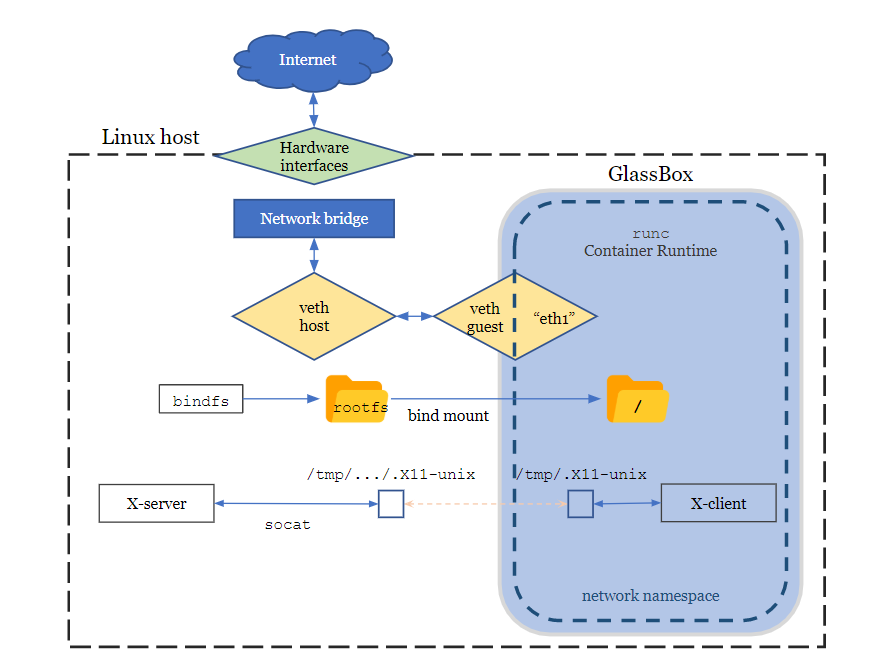
\includegraphics[width=0.5\textwidth]{architecture}
\caption{Architecture diagram}
\end{figure}

GlassBox provides an isolation mechanism that enables the creation of fault-tolerant host monitoring systems by providing host monitoring processes with a container that gives a read-only view of the host environment, targeted at exposing commonly monitored information such as CPU load, process information, memory usage, and network traffic. We configure this isolation mechanism in such a way that all requests to change the host's state, whether by modifications to the persistent data of the host filesystem or by modifications to volatile data in the host's memory outside the container, are blocked. Thus, this read-only container provides both of our criteria for a fault-tolerant host monitoring system: accurate view of the host state and strong guarantee of fault-tolerance.

In building our proof-of-concept, it made sense to extend runC to implement our read-only isolation, rather than building our own container, as runC is a well-established and well-tested example of a container runtime of the Open Container Initiative \cite{opencontainerinitiative}. Additionally, the runC component of GlassBox can be easily swapped out for a different container runtime such as LXC or rkt.

As we discovered through the use of the Linux utility \texttt{strace} in Section 4, most host-monitoring tools leverage special Linux virtual filesystem mounts (e.g. the \texttt{proc} mount on \texttt{/proc}) to read the information reported through these tools. This implies that the commonly monitored host information (e.g. CPU load, memory, etc.) can be extracted from within the container as long as the container can read the host's \texttt{/proc} directory.

Traditionally, network traffic can be monitored with utilities such as \texttt{tcpdump}, which hooks into a ``network tap'' in the kernel's network stack using Berkley Packet Filters (BPF) \cite{bsdpacketfilter}. For a container to gain the same network information by running an unmodified \texttt{tcpdump}, the host's network packets would have to be accessible inside the container as well, while any packets produced by the container must not be routable to any host applications.

Finally, many host monitoring applications are interactive and present user interfaces that organize the system information collected (examples include \textit{Wireshark} and \textit{GKrellM}). To maximize usability, our container should enable a method of viewing these graphical applications, even when running inside the container.

Given these observations and goals, our implementation of GlassBox focuses on four features: \textit{proces isolation}, \textit{read-only filesystem}, \textit{read-only networking}, and \textit{graphical display}. In the following subsections, we discuss the details of our implementation that provide these four features.

\subsection*{5.1 Process Isolation}

Process isolation is critical to GlassBox to provide necessary fault-containment. Our implementation provides this by instructing runC to create a \textit{pid namespace}, in which all container processes will start and execute. This ensures that processes in the container are unable to communicate directly with processes outside the container using standard inter-process communication methods such as signals and shared memory.

\subsection*{5.2 Read-Only Filesystem}

GlassBox require access to the host's full filesystem to launch host-monitoring processes, read from the \texttt{/proc} directory, and access monitored log files. We implement this through the use of the \texttt{bindfs} filesystem (built on FUSE) \cite{bindfs}, which presents a read-only userspace view of the host's full filesystem tree similar to a standard bind mount. By bind-mounting the host's root to the container root, we make the host root filesystem available inside the container, while by making the mount read-only, we prevent the container from modifying any of the host's files. Given access to the root file system, many tools like \texttt{top} can successfully collect statistics on the host, even when running inside GlassBox.

While a recursive bind mount using the \texttt{mount} utility can also present a read-only view of the host's full filesystem inside the container, but without the cost of trapping to userspace, we ultimately chose to use \texttt{bindfs}, despite the performance penalty, due to its userspace view of the host filesystem. This bypasses the complexity of working with the kernel's shared subtree semantics, as certain mount points can be labeled as ``unbindable'' \cite{mountman}.

Host-monitoring tools may write temporary log files to the filesystem. GlassBox configures an ephemeral mount point at the \texttt{/tmp} directory (a location commonly used by applications to store temporary data) via \texttt{tmpfs}, and uses \texttt{overlayfs} to overlay a second \texttt{tmpfs} over the user's home directory (commonly used by applications to store personalized configuration data). This ensures that applications that must write to disk can continue to function correctly, while the writes to the filesystem are ephemeral. Figure 5 shows the setup. The \texttt{overlay\_home} directory is the writeable upper directory, \texttt{overlay\_work} is the work directory used for preparing files between atomic actions. We create an overlay of \texttt{overlay\_home} on top of the bind-mounted root filesystem, to present a unified view of the upper directory (which is writeable) and the underlying root directory tree (which is read-only).

% can go on to discuss reading log files for applications that want to monitor other processes

\begin{figure}
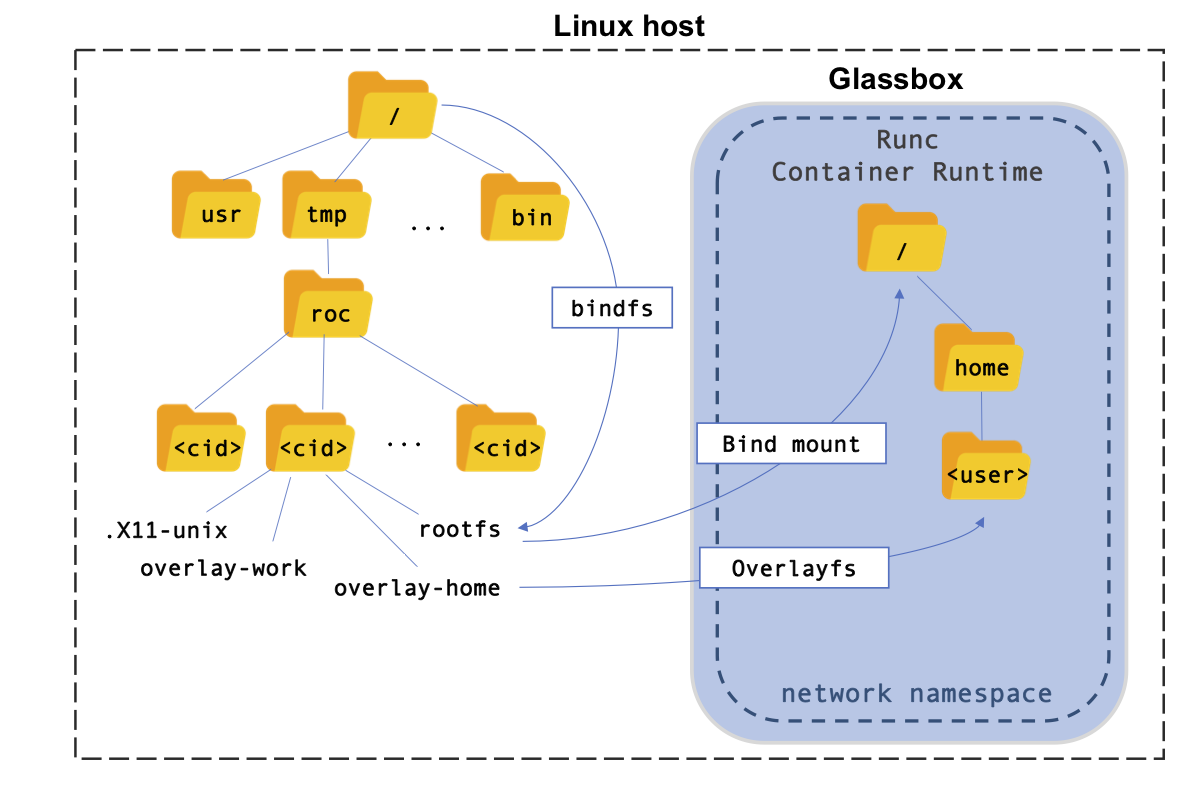
\includegraphics[width=0.5\textwidth]{fs_diagram}
\caption{Filesystem setup}
\end{figure}

\subsection*{5.3 Read-Only Networking}

GlassBox provides networking to containers via a bridge network. Each GlassBox instance has a network namespace to present the container its own network stack, routes, firewall rules, and network devices. Before the first container instance is launched, GlassBox creates the bridge network on the host and assigns an IP address. For each container, a Linux Virtual Ethernet (veth) device pair is created in the host network namespace. The host end of the pair is added to bridge network in the host network namespace, and the guest end is moved to the guest network namespace and added as an interface. The veth pair is a full duplex link, and thus acts as a tunnel between the bridge network and the guest network namespace. By default, the guest end of the veth pair is the only exposed interface in the container. Each guest-end of the veth pair is associated with an IP \texttt{192.168.10.<container id>}, where the id is a random integer between 0-255.

We create read-only behavior using \texttt{iptables} to restrict network packets. The \texttt{netfilter}/\texttt{iptables} utility uses a series of tables, each of which define firewall rules to filter or transform packets. To allow GlassBox to listen on the host's network traffic, we apply an iptables rule (\texttt{TEE}) that clones the packet and redirects it to our gateway IP. To prevent GlassBox processes from sending packets to (and potentially modifying the state of) the host, we specify the iptables rule (\texttt{DROP}) to drop outgoing packets. Thus, when multiple containers are connected to the same bridge network via veth pairs, each container cannot communicate with the host, nor with any other container.

Finally, runC provides configuration options for Linux capabilities to be set in a container. We set two capabilities by default, \texttt{CAP\_NET\_ADMIN} for listing all network interfaces, and \texttt{CAP\_NET\_RAW} to use raw sockets, which enable monitoring of network traffic.

One limitation of the networking setup is that the interfaces seen by GlassBox (for example, by running \texttt{ip addr}) are different from those seen by the host. We consider this discrepancy acceptable, since practically, host monitoring tools such as \texttt{tcpdump} and \textit{Wireshark} are interested in the network traffic rather than the the interfacs themselves. Since \texttt{TEE} clones the network packets, the IP source/destination appearing in packet captures still reflect the host interfaces.

\subsection*{5.4 Graphical Display}

GlassBox supports the execution of X11 applications inside the container and connects these processes with a display on the host. This enables users to launch full-graphical applications to visualize and interact with system information collected by host monitoring tools running from inside the container.

An X11 application reads from the environment variable \texttt{DISPLAY}, which contains three key pieces of information: \textit{hostname}, \textit{display number}, and \textit{screen number} \cite{xman}. When the hostname is specified, an X11 application tries to connect to that host's X server via TCP at the port number \texttt{6000 + <display number>}. When the hostname is not specified, the X11 application tries to connect to a Unix socket located at \texttt{/tmp/.X11-unix/X<display number>}.

GlassBox uses this X11 behavior to emulate an X server running inside the container and proxy the X11 connection to an X server running on the host. Before the container starts, GlassBox checks if a \texttt{DISPLAY} environment variable is set, and extracts the hostname. Assuming a \texttt{DISPLAY} variable exists, if there is no hostname, GlassBox assumes that the X server is running on the host and listening at the standard Unix socket location; otherwise, GlassBox assumes the X server is located at the host specified by \texttt{DISPLAY}. In either case, GlassBox will create a Unix socket file inside the container at \texttt{/tmp/.X11-unix/X<display number>} and uses the \texttt{socat} utility \cite{socatman} to bridge the Unix socket inside the container with the X server as defined by \texttt{DISPLAY}. A \texttt{DISPLAY} variable is then set inside the container to point to the newly-created Unix socket.

The X11 protocol also defines a way for a client to authenticate to a remote server using a \texttt{.Xauthority} file \cite{xsecurityman}, traditionally stored in a user's home directory. Without information stored in this file, an application inside the container cannot authenticate with the display server. GlassBox extracts the cookie stored inside the user's \texttt{.Xauthority} file that corresponds to the X server listed in \texttt{DISPLAY} and stores it in a \texttt{.Xauthority} file in the container's home directory. We use \texttt{overlayfs} to overlay this file over the home directory inside the container and avoid causing persistent modifications to the underlying filesystem data.

\section*{6. Evaluation}
We evaluated GlassBox on a range of host-monitoring and application performance monitoring tools, running on a virtualized Linux v4.9.0 environment. The host OS was macOS 10.4 and the hypervisor was VMware Fusion Professional Version 8.5.10. Figure 6 shows the tools on which we evaluated GlassBox, and any discrepancies between host and GlassBox outputs. The discrepancies are described and explained in the following subsections.
 \begin{figure}[h]
\begin{tabular}{ |p{35mm}|p{15mm}|p{20mm}| }
\hline
\textbf{Monitoring tool} &  \textbf{Resource} & \textbf{Differences}\\\hline
df (GNU coreutils) 8.26  & disk  &  due to\newline mounts\\\hline
du (GNU coreutils) 8.26  &  disk  &  due to\newline mounts\\\hline
ip (iproute2-ss161212) &  network & due to\newline network\newline namespace\\\hline
tcpdump 4.9.2&  network & minor\\\hline
free\newline from procps-ng 3.3.12 &  memory & none \\\hline
ps\newline from procps-ng 3.3.12 & process & minor\\\hline

pidstat \newline sysstat version 11.4.3 & process & minor \\\hline
sar \newline sysstat version 11.4.3 &  system activity & none\\\hline
gkrellm 2.3.10 & cpu, disk, \newline proc, net interfaces  & only net\newline interfaces \\\hline
Wireshark 2.6.7 & network & minor \\\hline
\end{tabular}
 \caption{Evaluation of monitoring tools running in GlassBox}
\end{figure}
\subsection*{6.1 \texttt{df} command}
The \texttt{df} command calls the \texttt{statfs()} system call to get statistics for a mounted filesystem, and as expected, shows different filesystems and mount points inside and outside the container. Due to the bind-mounting, the host root is shown as filesystem ``\texttt{/}'' mounted on ``\texttt{/}'' in GlassBox, while it is shown as filesystem ``\texttt{/dev/sda}'' mounted on ``\texttt{/}'' outside GlassBox. The bytes used and bytes available of the host root are consistent.
\subsection*{6.2 \texttt{ps} command}
Figure 7 shows the output from running \texttt{ps -a} inside and outside the container. The container displays \texttt{?} for the TTY since there are no terminals or pseudo-terminals attached to processes outside of the container. The full process tree (displayed with \texttt{ps -ajfwx}) reflects the place from which the \texttt{ps -ajfwx} process is launched. The the container output shows the \texttt{ps} process as a grandchild of the runc process, while the host shows the \texttt{ps} process at a higher level in the tree, directly as a child of a bash process outside the container. This discrepancy is minor since we do not expect a monitoring tool GlassBox to monitor its own bash shell and forked processes, or rely on its place in the process tree.
 \begin{figure}[h]
\begin{lstlisting}[linewidth=\linewidth]
  PID TTY          TIME CMD
  963 tty1     00:00:00 gnome-session-b
  986 tty1     00:00:12 gnome-shell
 1123 tty1     00:00:00 Xwayland
 1187 tty1     00:00:00 gnome-settings-
 1622 pts/1    00:00:00 start.sh
 1764 pts/1    00:00:00 sudo
 1765 pts/1    00:00:00 unshare
 1766 pts/1    00:00:00 launch_containe
 1838 pts/1    00:00:00 sudo
 1843 pts/1    00:00:00 socat
 1863 pts/1    00:00:00 runc
 2993 pts/0    00:00:00 ps
 \end{lstlisting}
\hspace{7.5em} a) outside GlassBox
 \begin{lstlisting}[linewidth=\linewidth]
  PID TTY          TIME CMD
  963 ?        00:00:00 gnome-session-b
  986 ?        00:00:12 gnome-shell
 1123 ?        00:00:00 Xwayland
 1187 ?        00:00:00 gnome-settings-
 1622 ?        00:00:00 start.sh
 1764 ?        00:00:00 sudo
 1765 ?        00:00:00 unshare
 1766 ?        00:00:00 launch_containe
 1838 ?        00:00:00 sudo
 1843 ?        00:00:00 socat
 1863 ?        00:00:00 runc
 2994 pts/0    00:00:00 ps
\end{lstlisting}
\hspace{7.5em} b) inside GlassBox
 \caption{\texttt{ps} output}
\end{figure}

\subsection*{6.3 \texttt{tcpdump} and Wireshark}
We ran tcpdump inside and outside a GlassBox instance to produce packet captures. There is a delay on the order of microseconds in packet timestamps in the capture inside GlassBox. Since the DNS resolver does not work in GlassBox, the packet capture shows ip addresses rather than domain names. The full packet capture is shown in Appendix B.

\subsection*{6.4 Evaluation Summary}

Our evaluation shows that a wide variety of monitoring tools can effectively monitor the host from inside GlassBox. We ran each monitoring tool without specifying specific pids, filesystems, or mounts, which produced extraneous output such as multiple tmpfs filesystems appearing in the \texttt{df} output. However, if we monitored a specific mount using  \texttt{df} or a specific directory using \texttt{du}, there would be no extraneous output.

\section*{7. GlassBox Performance}

%Include information about GlassBox experimental setup, including using tini as a lightweight userspace reaper to accurately track the container's process tree (since bindfs daemonizes)
We ran a preliminary memory profiler on GlassBox running in a Linux virtual machine. For our final results, we will run the profiler directly on a Linux machine, via Cloudlab. The memory profiler (Appendix A) traces memory usage across the launch of GlassBox, to the execution of \texttt{sleep 5} inside the container, and through the teardown of GlassBox. This execution spans across 15-20 executables that are called by GlassBox to set up the necessary namespaces, virtual network devices, X11 proxy, and others. runC itself requires 12 MB, and is the dominating memory cost. Other costs that remain consistent acrosss the execution of the container include the various structures we setup, such as the \texttt{bindfs} mount, and the \texttt{socat} connection between X11 server and client. Finally, many processes use memory during setup and teardown of the container.

We will also measure startup and execution overhead of GlassBox, using a runC container without GlassBox as a baseline. We expect these measurements to be somewhat implementation dependent on the container runtime, so it may be useful to measure GlassBox with other container runtimes such as LXC.

\section*{8. Future Work}
Future work could involve defining and implementing a more fine-grained security model. For example, specific syscall behaviors could be filtered through seccomp-bpf. Container resource usage could be restricted using cgroups. Refining the security model would require careful consideration, as we would want to maintain generality to be able to run a wide variety of tools.

We explored allowing GlassBox to monitor common applications that provide a specified API for ``read-only" status on a workload. A common use-case may be monitoring an application running inside a Docker instance. The Docker daemon manages a listening socket at \texttt{/var/run/docker.sock} as well as bridge network \texttt{docker0} to which containers are connected by default. We can configure the Docker daemon to listen on additional TCP, Unix, or fd socket endpoints, and expose these endpoints inside GlassBox.

Another solution would be to add GlassBox to the \texttt{docker0} bridge network the same way it was added to the \texttt{runc0} bridge using a veth pair. However, these solutions would depend on the Docker configuration, for example, the bridge solution would not work for networkless containers. Using sockets can work for any application that exposes a listening socket. For example, the \texttt{mytop} tool monitors the threads and overall performance of a MySQL server, with real-time queries/second statistics. It relies on the listening endpoint exposed by the MySQL Daemon, at \texttt{/var/run/mysqld/mysqld.sock}.

\section*{9. Conclusions}

%Include conclusions, mention there is more work to be done to improve the container and add additional features
With GlassBox, monitoring tools are able to run successfully and access host information in our container, with a high guarantee of fault tolerance. The implementation of GlassBox incurs some memory overhead, as shown by our profiling results. Even with these initial results, we expect that there is much future work that can be done to improve GlassBox and build new fault tolerant host monitoring systems.

\bibliographystyle{abbrv}
\bibliography{final-report}

\clearpage

\section*{Appendix A}

\AddToShipoutPicture*{
    \put(.5\paperwidth,.5\paperheight){\makebox(0,0){\includegraphics[scale=1]{memdata.eps}}}
}
\clearpage
\section*{Appendix B}
\begin{minipage}[t]{\textwidth}
Packet capture from downloading a file with \texttt{curl}, viewed in Wireshark inside GlassBox
\end{minipage}
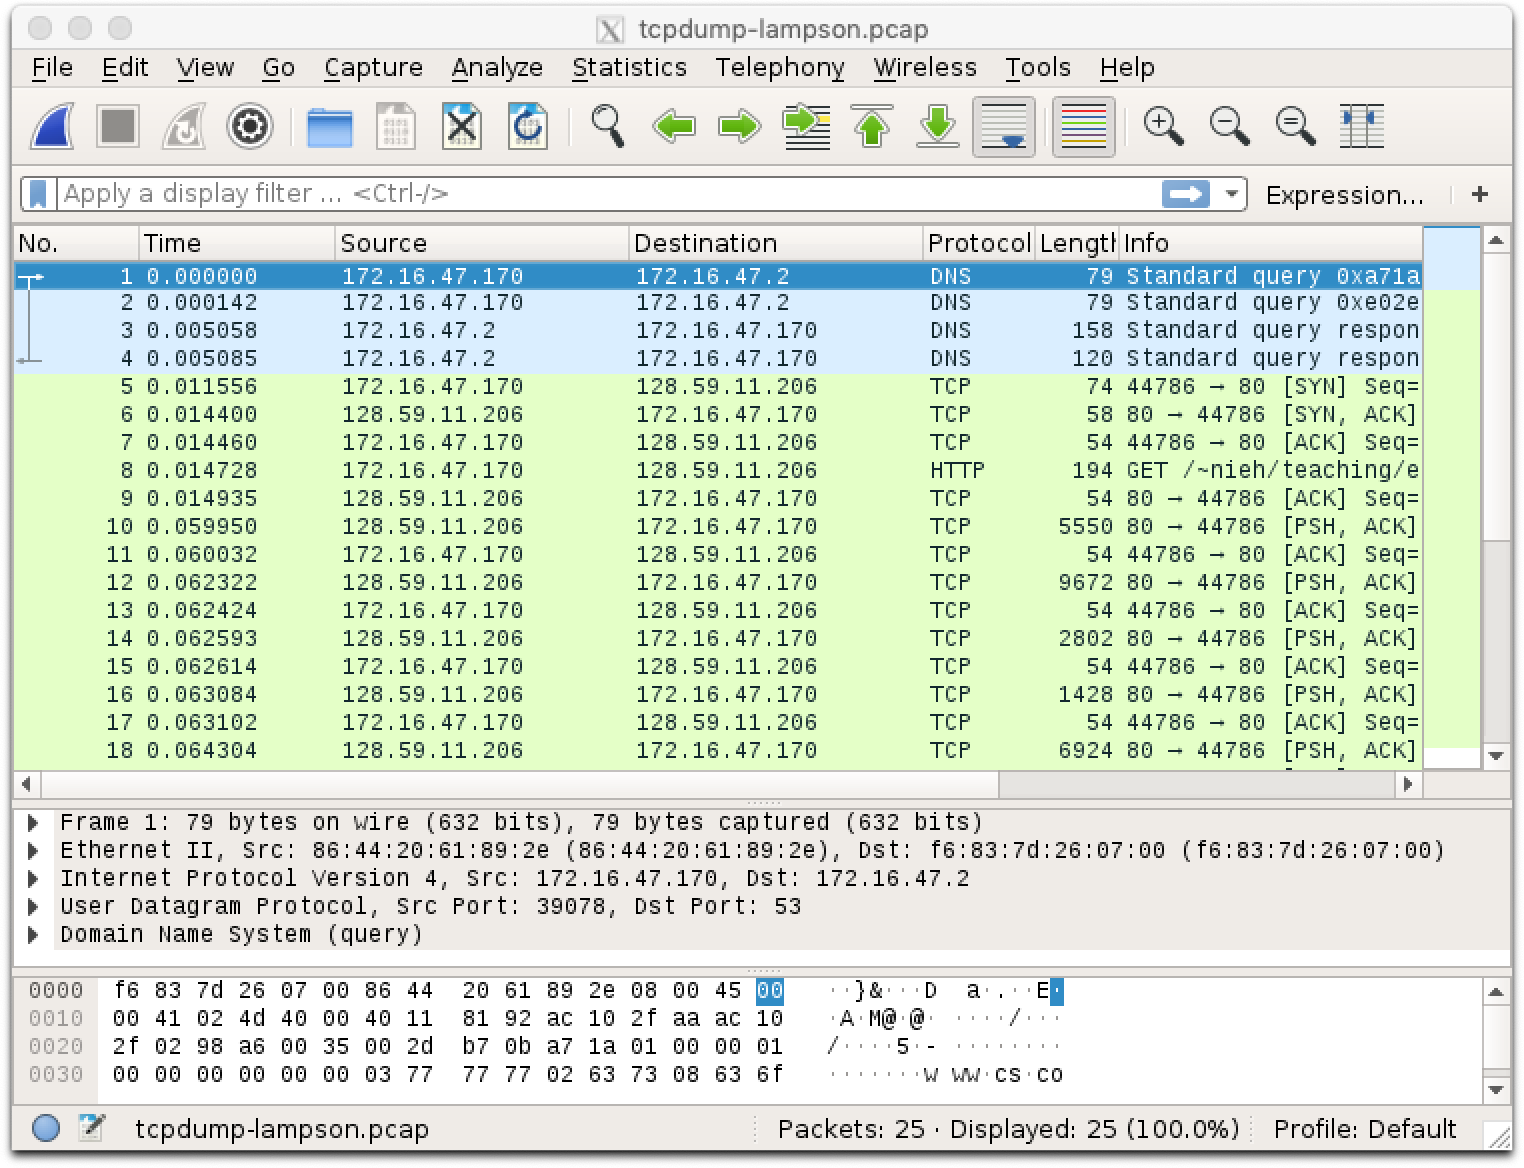
\includegraphics[scale=0.7]{wshark}
\clearpage
\begin{minipage}[t]{\textwidth}
Packet capture outside GlassBox
\begin{lstlisting}
reading from file tcpdump-lampson.pcap, link-type EN10MB (Ethernet)
2019-05-04 18:27:13.578649 IP w4118.44786 > webcluster.cs.columbia.edu.http: Flags [P.], seq 1:141, ack 1, win 29200, length 140: HTTP: GET /~nieh/teaching/e6118/papers/1_22_lampson_hints-design.pdf HTTP/1.1
2019-05-04 18:27:13.578856 IP webcluster.cs.columbia.edu.http > w4118.44786: Flags [.], ack 141, win 64240, length 0
2019-05-04 18:27:13.623871 IP webcluster.cs.columbia.edu.http > w4118.44786: Flags [P.], seq 1:5497, ack 141, win 64240, length 5496: HTTP: HTTP/1.1 200 OK
2019-05-04 18:27:13.623953 IP w4118.44786 > webcluster.cs.columbia.edu.http: Flags [.], ack 5497, win 39420, length 0
2019-05-04 18:27:13.626243 IP webcluster.cs.columbia.edu.http > w4118.44786: Flags [P.], seq 5497:15115, ack 141, win 64240, length 9618: HTTP
[trimmed]
2019-05-04 18:27:13.632915 IP webcluster.cs.columbia.edu.http > w4118.44786: Flags [P.], seq 34351:49465, ack 141, win 64240, length 15114: HTTP
2019-05-04 18:27:13.632945 IP w4118.44786 > webcluster.cs.columbia.edu.http: Flags [.], ack 49465, win 64240, length 0
\end{lstlisting}
Packet capture inside GlassBox
\begin{lstlisting}
reading from file tcpdump-lampson.pcap, link-type EN10MB (Ethernet)
2019-05-04 18:27:13.578655 IP 172.16.47.170.44786 > 128.59.11.206.http: Flags [P.], seq 1:141, ack 1, win 29200, length 140: HTTP: GET /~nieh/teaching/e6118/papers/1_22_lampson_hints-design.pdf HTTP/1.1
2019-05-04 18:27:13.578868 IP 128.59.11.206.http > 172.16.47.170.44786: Flags [.], ack 141, win 64240, length 0
2019-05-04 18:27:13.624088 IP 128.59.11.206.http > 172.16.47.170.44786: Flags [P.], seq 1:5497, ack 141, win 64240, length 5496: HTTP: HTTP/1.1 200 OK
2019-05-04 18:27:13.624106 IP 172.16.47.170.44786 > 128.59.11.206.http: Flags [.], ack 5497, win 39420, length 0
2019-05-04 18:27:13.626806 IP 128.59.11.206.http > 172.16.47.170.44786: Flags [P.], seq 5497:15115, ack 141, win 64240, length 9618: HTTP
[trimmed]
2019-05-04 18:27:13.633322 IP 128.59.11.206.http > 172.16.47.170.44786: Flags [P.], seq 34351:49465, ack 141, win 64240, length 15114: HTTP
2019-05-04 18:27:13.633339 IP 172.16.47.170.44786 > 128.59.11.206.http: Flags [.], ack 49465, win 64240, length 0
\end{lstlisting}
\end{minipage}

\end{document}
